\section{The Data}

The Data collected from the Hubble Space Telescope is for the star HD6268. The file extracted is a fits file, which is commonly used in Astrophysics and Astronomy.
Fits stands for Flexible Image Transport System, and is beneficial because it can store large amounts of data in a multi-dimensional array, as well a header and other information
related to the star such as date, sensor, position in the sky, etc. For star HD6268 the interest is in the wavelengths and their corresponding flux (or intensity).
The data sets are used to determine the abundances of different elements in the star. But, the data found in the fits file is raw data and must be formated. 


The first step is to extract the data from the fits file. This is simply done by using functions from the Astropy module in Python \cite{astropy}.
Two arrays are extracted; one being the wavelength and the other being the flux. Figure \ref{fig:raw_spec} is what the spectrum
looks like in its unaltered form.

\begin{figure}[h!]
\centering
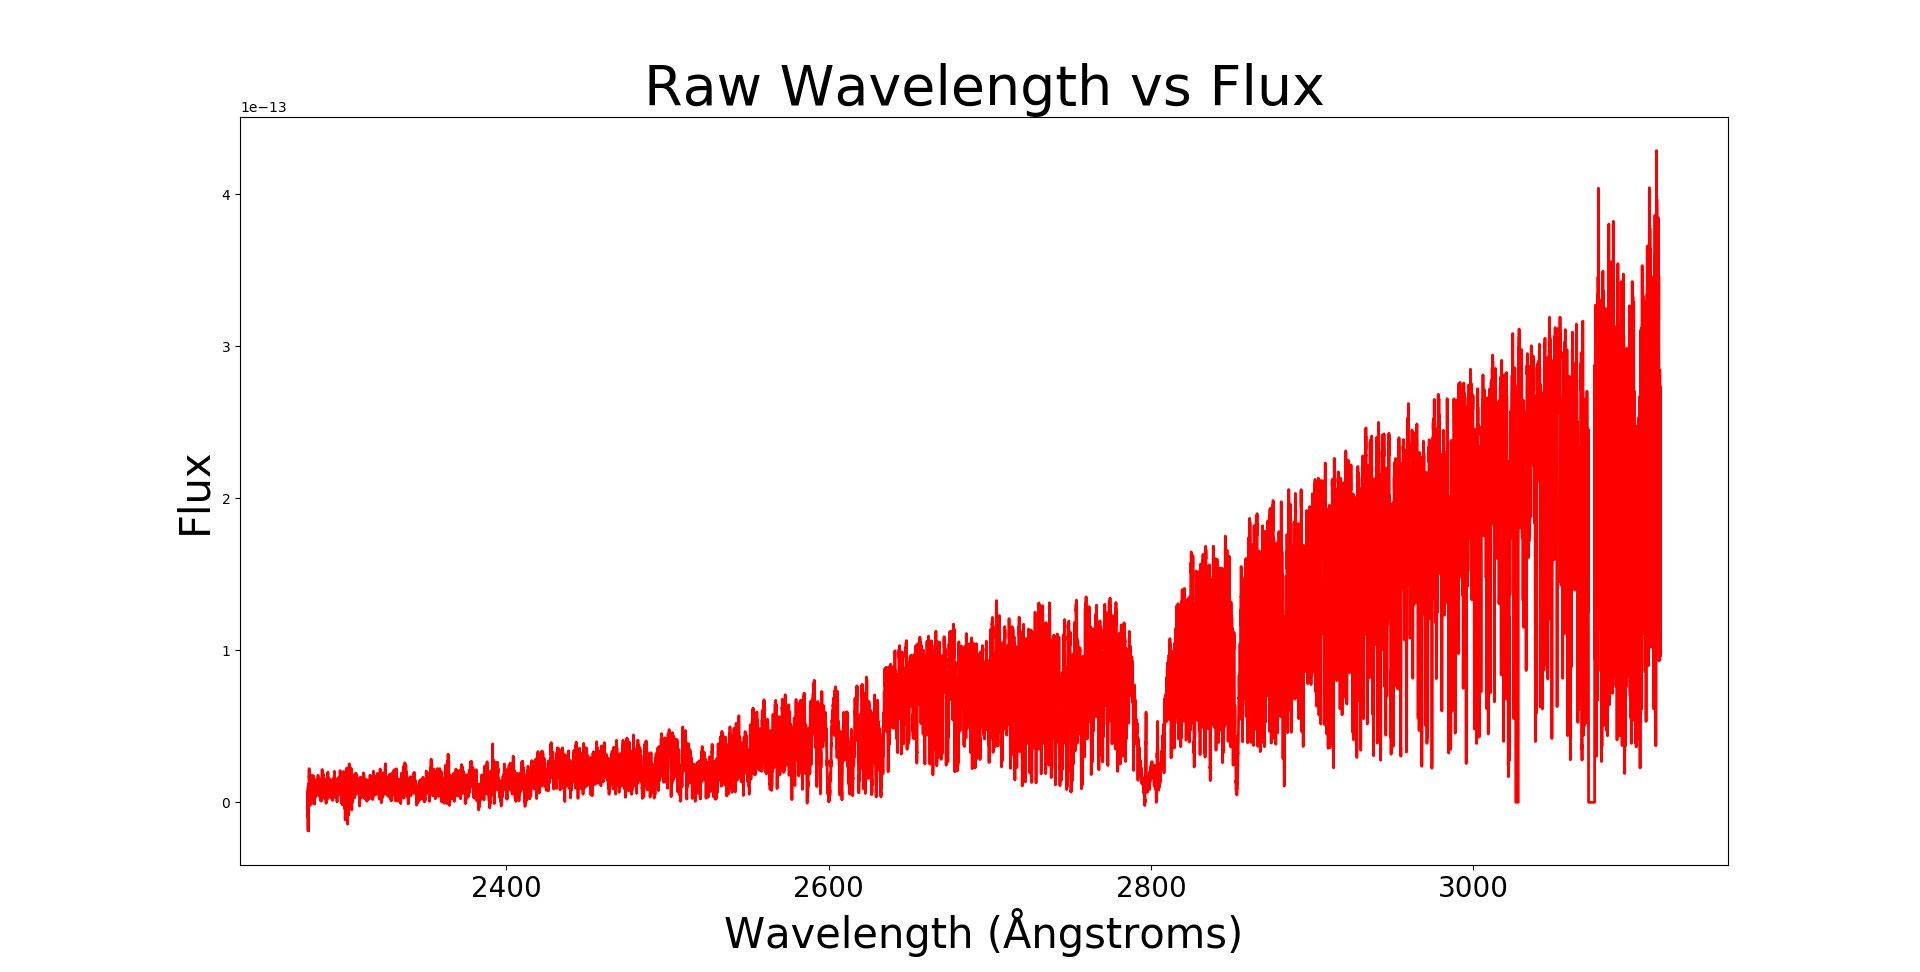
\includegraphics[width=\textwidth]{Raw_spectra.png}
\caption{Raw Spectrum of HD6268}
\label{fig:raw_spec}
\end{figure}


\section{Smoothing}
There is clearly a lot of noise that needs to be filtered out. Some causes for the noise are other nearby sensors or electronics,background radiation from other unknown cosmic sources (e.g cosmic rays), sensitivity of the sensors to certain wavelengths. To filter out the noise a method known as boxcar smoothing is applied here. The premise of boxcar smoothing is that in an array you go a certain amount of elements before and after the element that is being examined, and then average those elements to a single point. Then move to the next element in the array and repeat the process. Some data will be lost at the beginning and the end of the data set, but these data sets are so large that it should not matter. The following equation \ref{eq:boxcar}, from Mark Newman's textbook "Computational Physics" \cite{newman_computational_2013}, is used for the smoothing process.
The k value being the elemental position in the array, and the r value being how many elements you are summing before and after the current element you are at.

\begin{equation}
Y_k=\frac{1}{2r+1} \sum_{m=-r}^{m=+r} Y_{k+m}
\label{eq:boxcar}
\end{equation}


\begin{figure}[h!]
\centering
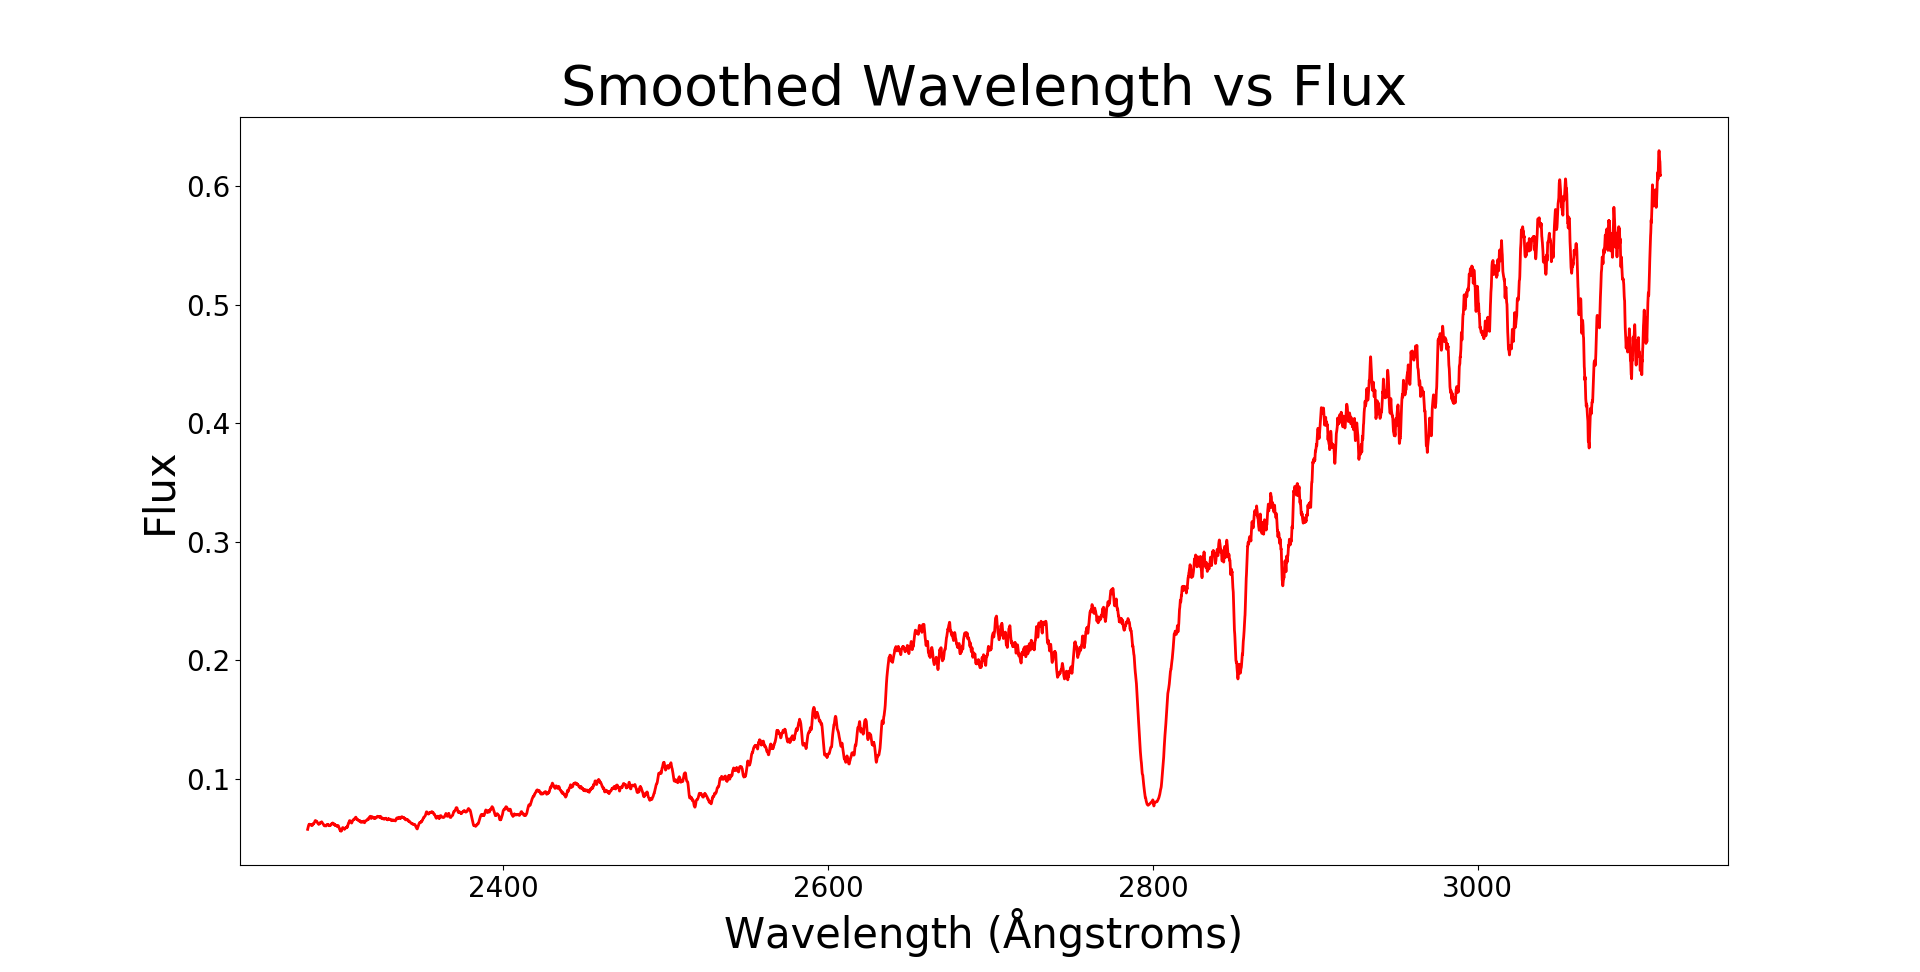
\includegraphics[width=\textwidth]{Smooth_spectra.png}
\caption{Smoothed Spectrum of HD6268}
\label{fig:smooth_spec}
\end{figure}


Figure \ref{fig:smooth_spec} is the process after running the smoothing function with a r value of 150. Comparing to Figure \ref{fig:raw_spec}, much of the features are easier to distinguish.
It is important that an appropriate r value is chosen; if the user chooses an r value that is too high than commonly the main features of the spectrum are eliminated.


\section{Normalizing}
Now for MOOG \cite{moog} to properly read the data, the data must be normalized between zero and one. To normalize the data we use a standard method in statistics to normalize the data.
Equation \ref{eq:norm} is used to normalize the function, with $x_{max}$ being the maximum value in an array and $x_{min}$ being the minimum \cite{stephanie_normalized_2015}.


\begin{equation}
X=\frac{x-x_{min}}{x_{max}-x_{min}}
\label{eq:norm}
\end{equation}

Running through the normalization procedure it can be seen in figure \ref{fig:norm_spec} there is a range of fluxes between zero and one.

\begin{figure}[h!]
\centering
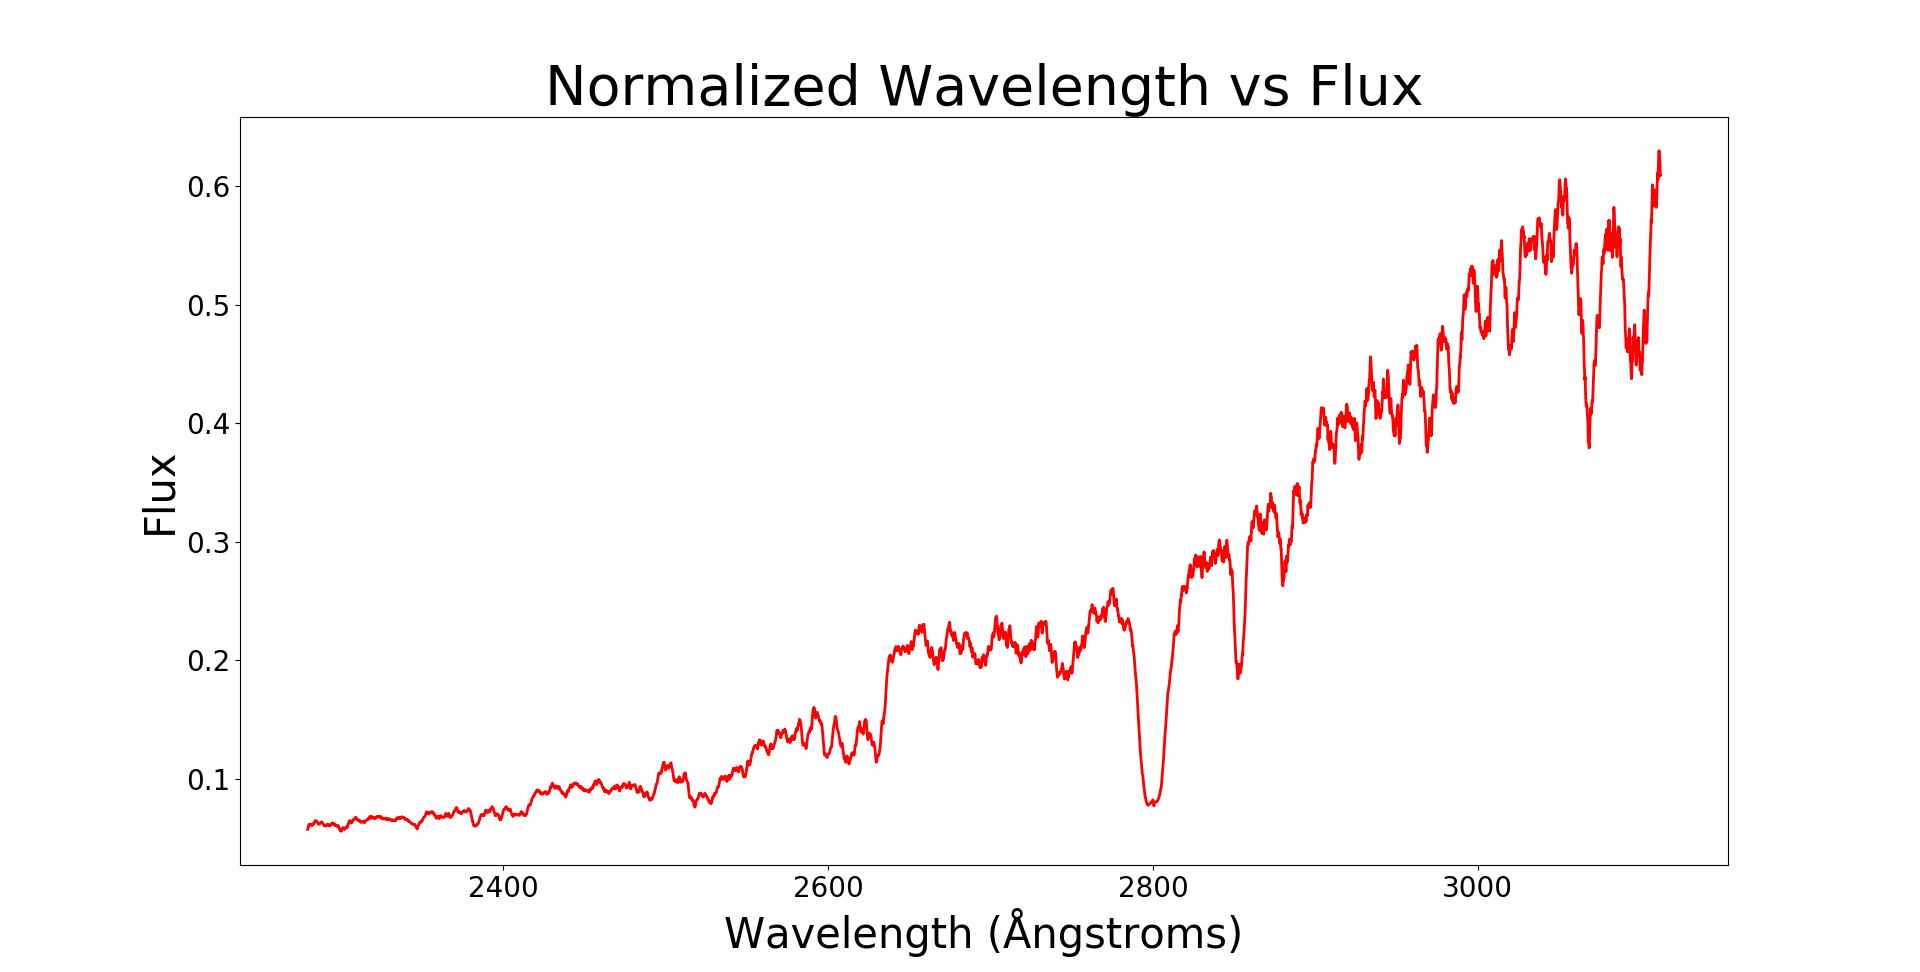
\includegraphics[width=\textwidth]{norm.png}
\caption{Normalized Spectrum of HD6268}
\label{fig:norm_spec}
\end{figure}


